\section{Activity: Sound from a Iron Rod / School Bell}
\subsection{Materials required}
\begin{enumerate}
\item A hanging iron rod or a school bell
\item A hammer
\end{enumerate}
\subsection{Procedure}
Strike the hanging iron rod/bell gently with the hammer. Listen to the sound produced. Touch the rod/bell gently with your finger. Do you feel any vibrations? Do you hear the bell ringing? Hold the rod/bell firmly with both hands and not let it move. Do you feel any vibrations now? Do you hear a buzzing sound?
\begin{marginfigure}
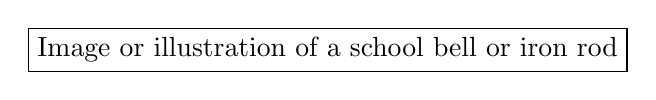
\begin{tikzpicture}
  \node[draw] at (0,0) {Image or illustration of a school bell or iron rod};
\end{tikzpicture}
  \caption{Image or illustration of a school bell or iron rod}
\end{marginfigure}
\subsection{Observe and record your observations}
\begin{fullwidth}
\begin{table}[h]
  \centering
  \begin{tabular}{lll}
    \toprule
    What you did & Did you feel any vibrations? & Did you hear a sound? \\
    \midrule
    Struck the bell and touched it gently & Yes / No &  Yes / No \\
    Held the bell firmly with both hands     & Yes / No &  Yes / No \\
    \bottomrule
  \end{tabular}
%   \caption{}
\end{table}
\end{fullwidth}

\newthought{Discuss} When did you hear the sound? When did the sound stop? What happened to the vibrations when you held the bell firmly?